\documentclass{article}
\usepackage[utf8]{inputenc}
\usepackage[T1]{fontenc}
\usepackage[english]{babel}
\setlength{\parindent}{0pt}
\usepackage{hyperref}
\hypersetup{
    colorlinks=true,
    linkcolor=blue,
    filecolor=magenta,      
    urlcolor=cyan}
\usepackage{graphicx}
\graphicspath{ {./pic/} }
\usepackage{multicol}
\usepackage{lscape}

\usepackage{fourier,amssymb,microtype,amsmath,gensymb}
\newcommand{\R}{\mathbb{R}}
\usepackage{mdframed,caption,xcolor}
\usepackage{tikz,tkz-euclide}

\title{Seminar 10. Incomplete Information in Dynamic Games}
\author{Xiaoguang Ling \\  \href{xiaoguang.ling@econ.uio.no}{xiaoguang.ling@econ.uio.no}}
\date{\today}

\begin{document}

\maketitle
 
%%%%%%%%%%%%%%%%%%%%%%%%%%%%%%%%%%%%%%%%%%%%%%%%%%%%%%%%%%%%%%%%%%%%%%%%%%%%%%%%%%%%%%%%%%%%%%
\section{Problem 1 - Screening and signaling}

Consider again the strategic situation described in Problem 1 of the set for the nineth seminar, 

\begin{center}
Game $1$ \vspace{6pt}

$
\begin{array}{c|c|c|}
 & L & R \\
\hline
U & 0,0 & 4,2 \\
\hline
D & 2,6 & 0,8 \\
\hline
\end{array}
$
\end{center}

\begin{center}
Game $2$ \vspace{6pt}

$
\begin{array}{c|c|c|}
 & L & R \\
\hline
U' & 0,2 & 0,0 \\
\hline
D' & 2,0 & 2,2 \\
\hline
\end{array}
$
\end{center}

where only player 1 knows which game is being played, while player 2 thinks that the two games are \textbf{equally likely}.


\subsection{(a) Screening} Assume now that \textbf{player 2 acts before player 1}, and that 2's choice can be observed by 1 before he makes his choice. Show that there is a unique subgame perfect Nash equilibrium. 

\begin{mdframed}[backgroundcolor=blue!20,linecolor=white]

Screening: Player \textbf{without} private information moves first $\Rightarrow$ there is nothing to infer (since player 1 knows everything, and player 2 has no chance to infer anything)

\begin{itemize}
\item Player 1 has private information: contingent strategy
\item Player 2 acts before player 1: can only choose between $L$ and $R$
\end{itemize}

\newpage

Extensive form:

\begin{center}
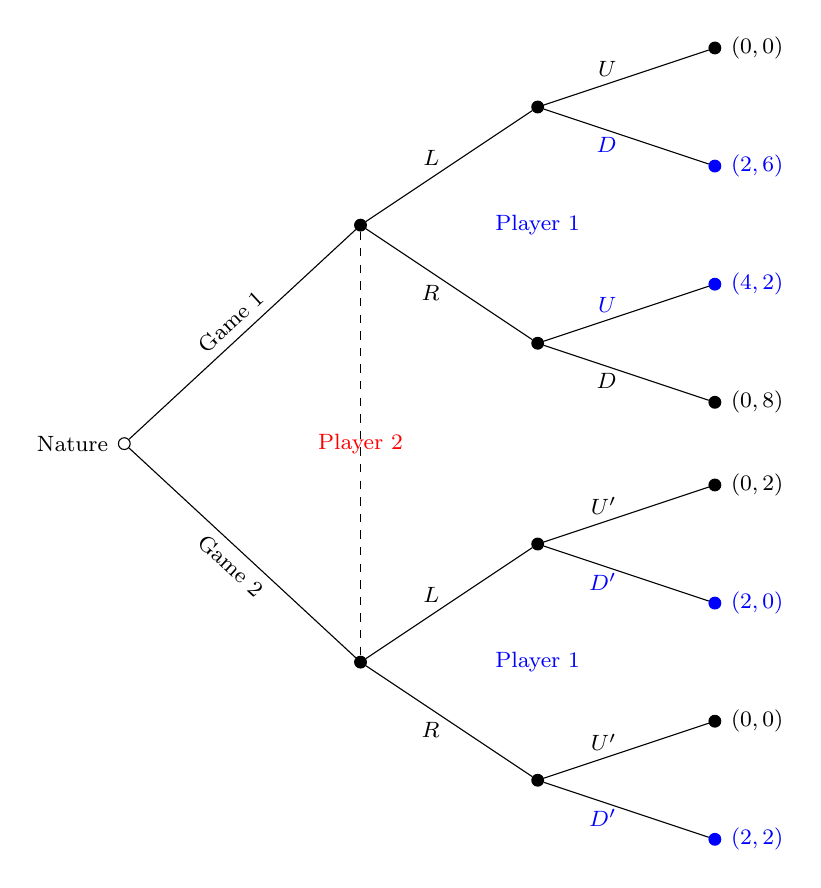
\begin{tikzpicture}[scale=1.5,font=\footnotesize]
\tikzset{
% Two node styles for game trees: solid and hollow
solid node/.style={circle,draw,inner sep=1.5,fill=black},
hollow node/.style={circle,draw,inner sep=1.5}
}
% Specify spacing for each level of the tree
\tikzstyle{level 1}=[level distance=20mm,sibling distance=37mm]
\tikzstyle{level 2}=[level distance=15mm,sibling distance=20mm]
\tikzstyle{level 3}=[level distance=15mm,sibling distance=10mm]
\tikzstyle arrowstyle=[scale=1]
\tikzstyle directed=[postaction={decorate,decoration={markings,
mark=at position .5 with {\arrow[arrowstyle]{stealth}}}}]

% The Tree
\node(0)[hollow node,label=left:{Nature}]{}[grow=east]
child{node(1)[solid node]{}
child{node(3)[solid node]{}
child{node[solid node,blue,label=right:{\textcolor{blue}{$(2,2)$}}]{}edge from parent node[left,blue,yshift=-3]{$D'$}}
child{node[solid node,label=right:{$(0,0)$}]{}edge from parent node[left,yshift=3]{$U'$}}
edge from parent node[left,yshift=-3]{$R$}}
child{node(4)[solid node]{}
child{node[solid node,blue,label=right:{\textcolor{blue}{$(2,0)$}}]{}edge from parent node[left,blue,yshift=-3]{$D'$}}
child{node[solid node,label=right:{$(0,2)$}]{}edge from parent node[left,yshift=3]{$U'$}}
edge from parent node[left,yshift=3]{$L$}
}
edge from parent node [midway, below, sloped] (TextNode) {Game 2}
}
child{node(2)[solid node]{}
child{node(5)[solid node]{}
child{node[solid node,label=right:{$(0,8)$}]{}edge from parent node[left,yshift=-3]{$D$}}
child{node[solid node,blue,label=right:{\textcolor{blue}{$(4,2)$}}]{}edge from parent node[left,blue,yshift=3]{$U$}}
edge from parent node[left,yshift=-3]{$R$}}
child{node(6)[solid node]{}
child{node[solid node,blue,label=right:{\textcolor{blue}{$(2,6)$}}]{}edge from parent node[left,blue,yshift=-3]{$D$}}
child{node[solid node,label=right:{$(0,0)$}]{}edge from parent node[left,yshift=3]{$U$}}
edge from parent node[left,yshift=3]{$L$}
}
edge from parent node [midway, above, sloped] (TextNode) {Game 1}
};
% information set
\draw [dashed] (2) -- (1) ;
% specify mover
\node at ($(1)!.5!(2)$) {\textcolor{red}{Player 2}};
\node at ($(5)!.5!(6)$) {\textcolor{blue}{Player 1}};
\node at ($(3)!.5!(4)$) {\textcolor{blue}{Player 1}};
\end{tikzpicture}
\end{center}

Player 1 acts contingently; Player 2 acts according to the expected payoff based on some belief $(\tfrac12,\tfrac12)$; 
\begin{itemize}
\item Note: use backward induction method to calculate player 2's expected payoff (payoff in blue)
\item We can also find when Game 2 is played, for player 1, $D'$ dominates $U'$
\end{itemize}

The contingent strategy for player 1 is easy to express, since there is no incomplete information.

\end{mdframed}

The strategy of player 1:
\begin{itemize}
\item If Game 1 is played:
\begin{itemize}
\item when player 2 chooses $L$, player 1 chooses $D$
\item when player 2 chooses $R$, player 1 chooses $U$
\end{itemize}
\item If Game 2 is played:
\begin{itemize}
\item when player 2 chooses $L$, player 1 chooses $D'$
\item when player 2 chooses $R$, player 1 chooses $D'$
\end{itemize}
\end{itemize}

For player 2:


$$E(U^2_L) = \tfrac12 \times 6 +\tfrac12 \times 0 = 3$$
$$E(U^2_R) = \tfrac12 \times 2 +\tfrac12 \times 2 = 2$$
$$\Rightarrow E(U^2_L) > E(U^2_R)$$

The strategy of player 2 is to choose $L$.

\medskip

Therefore there is only one SPNE:

\{(For player 1) In Game 1: $D$ after $L$, $U$ after $R$. In Game 2, $D'$ after $L$, $D'$ after $R$ ; (For player 2) $L$\}


\subsection{(b) Signaling} Assume now that player 1 acts before player 2, and that 1's choice can be observed by 2 before she makes her choice. Show that there is a unique separating perfect Bayesian equilibrium.

\bigskip


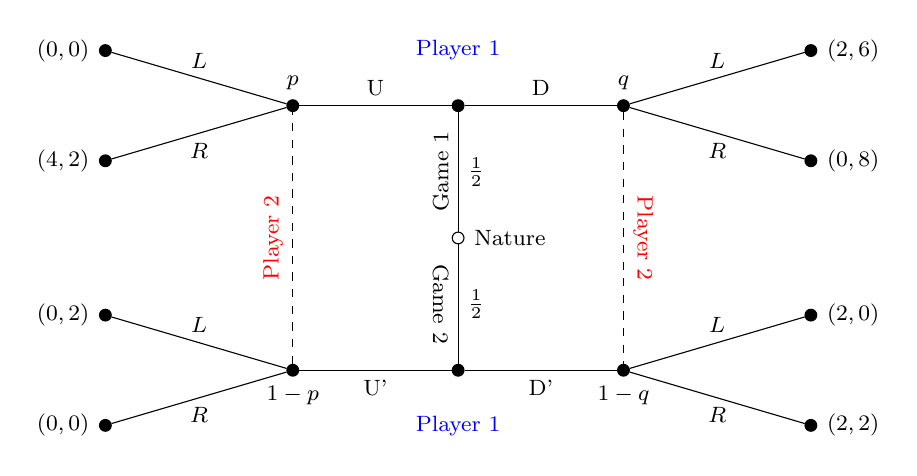
\begin{tikzpicture}[scale=1.4,font=\footnotesize]
\tikzset{
% Two node styles for game trees: solid and solid
solid node/.style={circle,draw,inner sep=1.5,fill=black},
hollow node/.style={circle,draw,inner sep=1.5}}
% Specify spacing for each level of the tree
\tikzstyle{level 1}=[level distance=12mm,sibling distance=25mm]
\tikzstyle{level 2}=[level distance=15mm,sibling distance=15mm]
\tikzstyle{level 3}=[level distance=17mm,sibling distance=10mm]
% The Tree
\node(0)[hollow node,label=right:{Nature}]{}
child[grow=up]{node[solid node,label=above:{
\begin{tabular}{c}
\textcolor{blue}{Player 1} \\ \\
\end{tabular}}] {}
child[grow=left]{node(1)[solid node,label=above:{$p$}]{}
child{node[solid node,label=left:{$(0,0)$}]{} edge from parent node [above]{$L$}}
child{node[solid node,label=left:{$(4,2)$}]{} edge from parent node [below]{$R$}}
edge from parent node [above]{U}}
child[grow=right]{node(3)[solid node,label=above:{$q$}]{}
child{node[solid node,label=right:{$(0,8)$}]{} edge from parent node [below]{$R$}}
child{node[solid node,label=right:{$(2,6)$}]{} edge from parent node [above]{$L$}}
edge from parent node [above]{D}
}
edge from parent node [right]{$\tfrac12$} node [midway, above, sloped] (TextNode){Game 1}
}
child[grow=down]{node[solid node,label=below:{\begin{tabular}{c}
\\ \textcolor{blue}{Player 1}
\end{tabular}}] {}
child[grow=left]{node(2)[solid node,label=below:{$1-p$}]{}
child{node[solid node,label=left:{$(0,2)$}]{} edge from parent node [above]{$L$}}
child{node[solid node,label=left:{$(0,0)$}]{} edge from parent node [below]{$R$}}
edge from parent node [below]{U'}
}
child[grow=right]{node(4)[solid node,label=below:{$1-q$}]{}
child{node[solid node,label=right:{$(2,2)$}]{} edge from parent node [below]{$R$}}
child{node[solid node,label=right:{$(2,0)$}]{} edge from parent node [above]{$L$}}
edge from parent node [below]{D'}
}
edge from parent node [right]{$\tfrac12$} node[midway, below, sloped] (TextNode){Game 2}
};
% information set
\draw [dashed] (2) -- (1) node [midway, above, sloped, red] (TextNode) {Player 2};
\draw [dashed] (3) -- (4) node [midway, above, sloped, red] (TextNode) {Player 2};
\end{tikzpicture}

















\section{Problem 2 - Sequential moves and incomplete information; Perfect
Bayesian equilibrium}

Consider the situation of Problem 1 of the eighth seminar, but assume now in addition that the pizza comes in 5
different sizes, each with $x$ slices, where $x \in \{4, 6, 8, 10, 12\}$. Player 1 observes $x$
before making her demand, while players 2 only observes player 1's demand, but not $x$, before
having to make his own demand. Before observing player 1's demand, player 2 thinks that the 5
different pizza sizes are equally likely, but he may infer something from her demand.
%

%
\subsection{(a) Explain what a strategy is for player 1 in this game of incomplete information.} 
%
\subsection{(b) perfect Bayesian
equilibrium} Show that the following strategy for player 1 can be part of a perfect Bayesian
equilibrium: $s_1(4) = 2$, $s_1(6) = 3$, $s_1(8) = 4$, $s_1(10) = 5$, $s_1(12) = 11$. Specify
both player 2's strategy and player 2's beliefs. 
%
\subsection{(c) Are there other perfect Bayesian equilibria in this game?} %


\bigskip

\section{Problem 3 - Challenging an incumbent}

Consider a market where there is an incumbent firm and a challenger. The challenger is
\textit{strong} with probability $\tfrac12$ and \textit{weak} with probability $\tfrac12$; it knows its type, but the incumbent
does not. The challenger may either \textit{prepare} itself for battle or remain \textit{unprepared}. The
incumbent observes the challenger's preparedness, but not its type, and chooses whether to
\textit{fight} ($F$) or \textit{acquiesce} ($A$). The extensive form and the payoffs are given by the following
figure. The challenger's payoff is listed first, the incumbent's second.


\bigskip

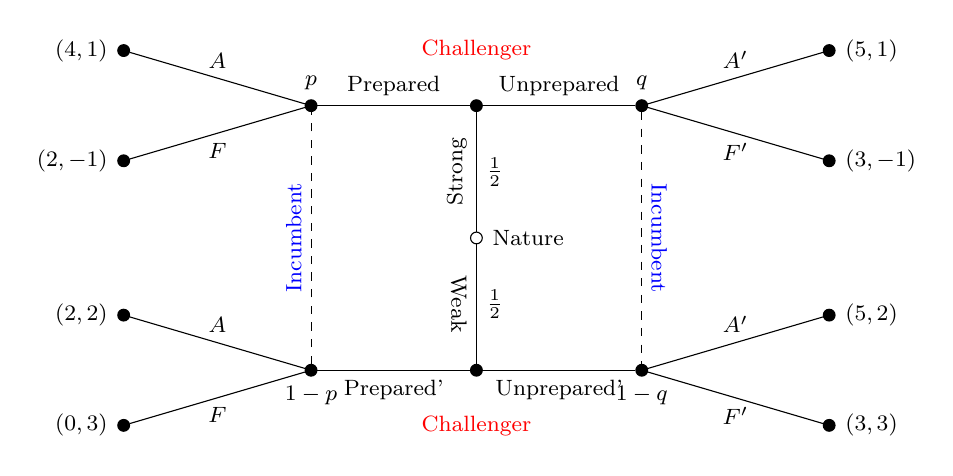
\begin{tikzpicture}[scale=1.4,font=\footnotesize]
\tikzset{
% Two node styles for game trees: solid and solid
solid node/.style={circle,draw,inner sep=1.5,fill=black},
hollow node/.style={circle,draw,inner sep=1.5}}
% Specify spacing for each level of the tree
\tikzstyle{level 1}=[level distance=12mm,sibling distance=25mm]
\tikzstyle{level 2}=[level distance=15mm,sibling distance=15mm]
\tikzstyle{level 3}=[level distance=17mm,sibling distance=10mm]
% The Tree
\node(0)[hollow node,label=right:{Nature}]{}
child[grow=up]{node[solid node,label=above:{
\begin{tabular}{c}
\textcolor{red}{Challenger} \\ \\
\end{tabular}}] {}
child[grow=left]{node(1)[solid node,label=above:{$p$}]{}
child{node[solid node,label=left:{$(4,1)$}]{} edge from parent node [above]{$A$}}
child{node[solid node,label=left:{$(2,-1)$}]{} edge from parent node [below]{$F$}}
edge from parent node [above]{Prepared}}
child[grow=right]{node(3)[solid node,label=above:{$q$}]{}
child{node[solid node,label=right:{$(3,-1)$}]{} edge from parent node [below]{$F'$}}
child{node[solid node,label=right:{$(5,1)$}]{} edge from parent node [above]{$A'$}}
edge from parent node [above]{Unprepared}
}
edge from parent node [right]{$\tfrac12$} node [midway, above, sloped] (TextNode){Strong}
}
child[grow=down]{node[solid node,label=below:{\begin{tabular}{c}
\\ \textcolor{red}{Challenger}
\end{tabular}}] {}
child[grow=left]{node(2)[solid node,label=below:{$1-p$}]{}
child{node[solid node,label=left:{$(2,2)$}]{} edge from parent node [above]{$A$}}
child{node[solid node,label=left:{$(0,3)$}]{} edge from parent node [below]{$F$}}
edge from parent node [below]{Prepared'}
}
child[grow=right]{node(4)[solid node,label=below:{$1-q$}]{}
child{node[solid node,label=right:{$(3,3)$}]{} edge from parent node [below]{$F'$}}
child{node[solid node,label=right:{$(5,2)$}]{} edge from parent node [above]{$A'$}}
edge from parent node [below]{Unprepared'}
}
edge from parent node [right]{$\tfrac12$} node[midway, below, sloped] (TextNode){Weak}
};
% information set
\draw [dashed] (2) -- (1) node [midway, above, sloped, blue] (TextNode) {Incumbent};
\draw [dashed] (3) -- (4) node [midway, above, sloped, blue] (TextNode) {Incumbent};
\end{tikzpicture}

\medskip

\subsection{(a) What are the (pure) strategies for the challenger?} 



\subsection{(b) Why is there no perfect Bayesian equilibrium where the weak challenger chooses
\textit{Prepared}$'$ ? }


\subsection{(c) Separating}Show that there is a perfect Bayesian equilibrium where the strong challenger chooses
\textit{Prepared} and the weak challenger chooses \textit{Unprepared}$'$. 


\subsection{(d) Pooling}Show that there is a perfect Bayesian equilibrium where the strong challenger chooses
\textit{Unprepared} and the weak challenger chooses \textit{Unprepared}$'$. What do we call such an
equilibrium? 






\end{document}
